% Options for packages loaded elsewhere
\PassOptionsToPackage{unicode}{hyperref}
\PassOptionsToPackage{hyphens}{url}
%
\documentclass[
  x11names]{article}
\usepackage{amsmath,amssymb}
\usepackage{lmodern}
\usepackage{iftex}
\ifPDFTeX
  \usepackage[T1]{fontenc}
  \usepackage[utf8]{inputenc}
  \usepackage{textcomp} % provide euro and other symbols
\else % if luatex or xetex
  \usepackage{unicode-math}
  \defaultfontfeatures{Scale=MatchLowercase}
  \defaultfontfeatures[\rmfamily]{Ligatures=TeX,Scale=1}
\fi
% Use upquote if available, for straight quotes in verbatim environments
\IfFileExists{upquote.sty}{\usepackage{upquote}}{}
\IfFileExists{microtype.sty}{% use microtype if available
  \usepackage[]{microtype}
  \UseMicrotypeSet[protrusion]{basicmath} % disable protrusion for tt fonts
}{}
\makeatletter
\@ifundefined{KOMAClassName}{% if non-KOMA class
  \IfFileExists{parskip.sty}{%
    \usepackage{parskip}
  }{% else
    \setlength{\parindent}{0pt}
    \setlength{\parskip}{6pt plus 2pt minus 1pt}}
}{% if KOMA class
  \KOMAoptions{parskip=half}}
\makeatother
\usepackage{xcolor}
\usepackage[margin=1in]{geometry}
\usepackage{graphicx}
\makeatletter
\def\maxwidth{\ifdim\Gin@nat@width>\linewidth\linewidth\else\Gin@nat@width\fi}
\def\maxheight{\ifdim\Gin@nat@height>\textheight\textheight\else\Gin@nat@height\fi}
\makeatother
% Scale images if necessary, so that they will not overflow the page
% margins by default, and it is still possible to overwrite the defaults
% using explicit options in \includegraphics[width, height, ...]{}
\setkeys{Gin}{width=\maxwidth,height=\maxheight,keepaspectratio}
% Set default figure placement to htbp
\makeatletter
\def\fps@figure{htbp}
\makeatother
\setlength{\emergencystretch}{3em} % prevent overfull lines
\providecommand{\tightlist}{%
  \setlength{\itemsep}{0pt}\setlength{\parskip}{0pt}}
\setcounter{secnumdepth}{-\maxdimen} % remove section numbering
\usepackage{fontspec} \usepackage{titling} \pretitle{\begin{center} \vspace{-3cm}
\includegraphics[width=\linewidth]{images/Base_info/logo.png}\LARGE\\} \posttitle{\end{center}} \usepackage{float} \usepackage{fancyhdr} \usepackage{ragged2e} \usepackage{caption} \usepackage{colortbl} \captionsetup[figure]{labelformat=empty} \arrayrulecolor{white} \pagestyle{fancy} \fancyhead[L,C]{} \fancypagestyle{plain}{\pagestyle{fancy}} \PassOptionsToPackage{dvipsnames,svgnames*,x11names*}{xcolor} \definecolor{ceil}{rgb}{0.57, 0.63, 0.81}
\usepackage{booktabs}
\usepackage{longtable}
\usepackage{array}
\usepackage{multirow}
\usepackage{wrapfig}
\usepackage{float}
\usepackage{colortbl}
\usepackage{pdflscape}
\usepackage{tabu}
\usepackage{threeparttable}
\usepackage{threeparttablex}
\usepackage[normalem]{ulem}
\usepackage{makecell}
\usepackage{xcolor}
\ifLuaTeX
  \usepackage{selnolig}  % disable illegal ligatures
\fi
\IfFileExists{bookmark.sty}{\usepackage{bookmark}}{\usepackage{hyperref}}
\IfFileExists{xurl.sty}{\usepackage{xurl}}{} % add URL line breaks if available
\urlstyle{same} % disable monospaced font for URLs
\hypersetup{
  pdftitle={Blastocerus dichotomus},
  hidelinks,
  pdfcreator={LaTeX via pandoc}}

\title{\emph{Blastocerus dichotomus}}
\usepackage{etoolbox}
\makeatletter
\providecommand{\subtitle}[1]{% add subtitle to \maketitle
  \apptocmd{\@title}{\par {\large #1 \par}}{}{}
}
\makeatother
\subtitle{\textbf{Ciervo de los pantanos}}
\author{}
\date{\vspace{-2.5em}Fecha de creación: 03 April, 2023}

\begin{document}
\maketitle

\setmainfont{Calibri}
\setsansfont{Calibri}
\setmonofont{Calibri}

\newcommand\invisiblesection[1]{%
  \refstepcounter{section}%
  \addcontentsline{toc}{section}{\protect\numberline{\thesection}#1}%
  \sectionmark{#1}}

\fancyhead[R]{\textbf{http://doi.org/10.31687/SaremLR.19.207}}

%
  \refstepcounter{section}%
  \addcontentsline{toc}{section}{\protect\numberline{\thesection}GENERALIDADES}%
  \sectionmark{GENERALIDADES}
<<<<<<< HEAD
\vspace{-0.4cm}
=======
>>>>>>> e88e2e6dc178d3b716c81e431bc0d17dd25cb694

\center

\textbf{Autores: Pereira, Javier A.; Varela, Diego; Aprile, Gustavo;
Cirignoli, Sebastián; Orozco, María Marcela; Lartigau, Bernardo; De
Angelo, Carlos; Giraudo, Alejandro R.}

\begin{figure}[H]

{\centering 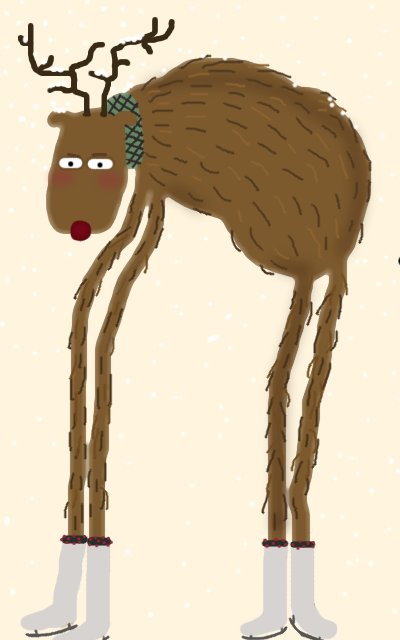
\includegraphics[width=0.35\linewidth]{photos/Blastocerus dichotomus} 

}

\caption{Fotos por Salvador Dali}\label{fig:image}
\end{figure}

\begin{center}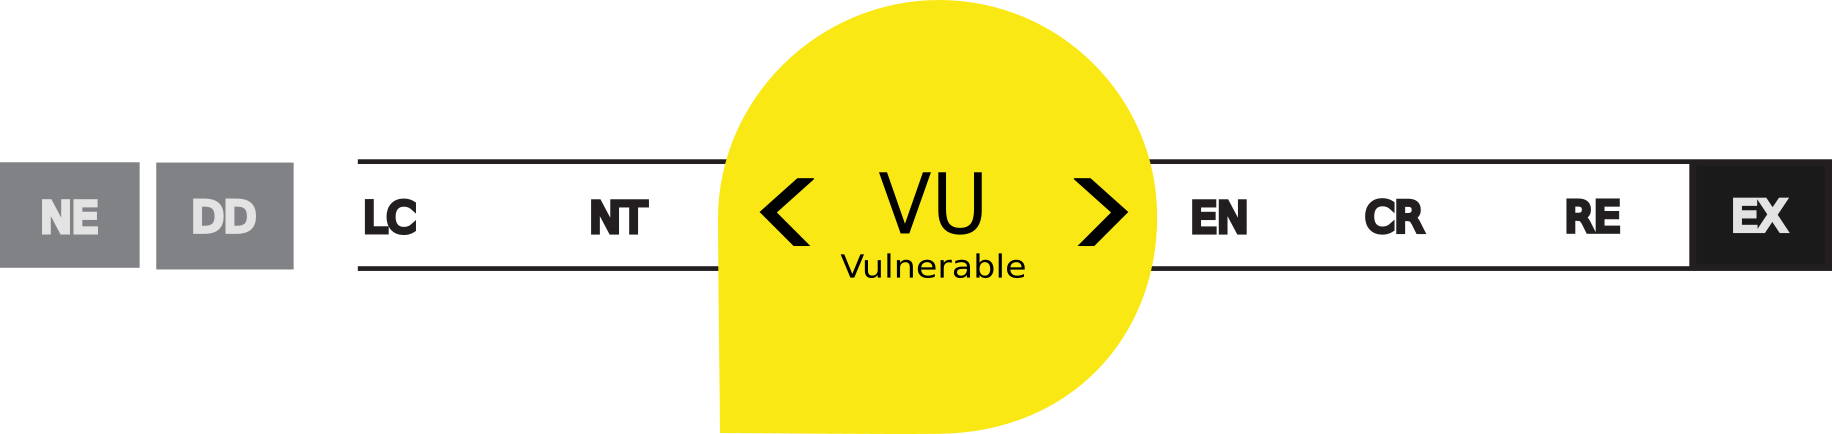
\includegraphics[width=0.7\linewidth]{images/scale-vu} \end{center}

\begin{center}\rule{0.5\linewidth}{0.5pt}\end{center}

\justifying

\textbf{Citar como:} Pereira, Javier A.; Varela, Diego; Aprile, Gustavo;
Cirignoli, Sebastián; Orozco, María Marcela; Lartigau, Bernardo; De
Angelo, Carlos; Giraudo, Alejandro R.. (2019). \emph{Blastocerus
dichotomus}. En: SAyDS--SAREM (eds.) Categorización 2019 de los
mamíferos de Argentina según su riesgo de extinción. Lista Roja de los
mamíferos de Argentina. Versión digital: \url{http://cma.sarem.org.ar}.

\begin{center}\rule{0.5\linewidth}{0.5pt}\end{center}

\newpage

%
  \refstepcounter{section}%
  \addcontentsline{toc}{section}{\protect\numberline{\thesection}CATEGORÍAS DE CONSERVACIÓN}%
  \sectionmark{CATEGORÍAS DE CONSERVACIÓN}
\begin{table}[H]
\centering
\begin{tabular}[t]{>{\raggedright\arraybackslash}m{16cm}>{}m{16cm}}
\toprule
\cellcolor{ceil}{\textcolor{white}{\textbf{\rule{0pt}{14pt}CATEGORÍAS DE CONSERVACIÓN}}}\\
\bottomrule
\end{tabular}
\end{table}

\vspace{-0.4cm}

\textbf{Categoría Nacional de Conservación 2019}

VU (Vulnerable)

\textbf{Criterios y subcriterios}

A3cde

\textbf{Justificación de la categorización}

El ciervo de los pantanos es una especie dependiente de ambientes de
humedales y está sujeto a una alta presión de caza furtiva. Su rango de
distribución se encuentra fragmentado en al menos cuatro subpoblaciones.
Si bien la subpoblación de los Esteros del Iberá y áreas adyacentes, en
la provincia de Corrientes, ha experimentado una importante recuperación
en los últimos 30 años, el resto de las subpoblaciones se encuentran
amenazadas (ver Evaluación de Subpoblaciones). La caza furtiva y el
drenaje de los humedales para la producción agropecuaria, forestaciones
y urbanizaciones son sus principales amenazas. La especie se ve afectada
por las inundaciones extraordinarias que provocan mortalidades masivas
por aumento en la presión de cacería, desnutrición, enfermedades y
temperaturas extremas. Algunas subpoblaciones también se encuentran
amenazadas por el ataque de perros, la competencia por interferencia con
el ganado bovino y el atropellamiento en rutas. A nivel nacional, la
especie está categorizada como Vulnerable (VU) con una proyección de
reducción de su tamaño poblacional del 30\% hacia el futuro (15 años,
tres generaciones), teniendo en cuenta la reducción del EOO, AOO y la
calidad de hábitat, y los impactos de la caza furtiva y de las
inundaciones extraordinarias (incrementadas por el cambio climático).

\textbf{Evaluación de subpoblaciones locales}

\begin{tabu} to \linewidth {>{\raggedright}X>{\raggedright}X>{\raggedright}X}
\toprule
\textbf{Subpoblación} & \textbf{Categoría} & \textbf{Criterios y subcriterios}\\
\arrayrulecolor{white}
\midrule
\cellcolor{gray!6}{Esteros del Iberá y áreas aledañas} & \cellcolor{gray!6}{NT (Casi Amenazada)} & \cellcolor{gray!6}{C}\\
\bottomrule
\end{tabu}

\textbf{Justificación}

Los Esteros del Iberá y sus adyacencias albergan el mayor número de
ciervos de los pantanos de la Argentina. Durante el último relevamiento
poblacional realizado en parte de la Reserva Iberá se estimaron unos
6.000 ejemplares (De Angelo et al.~2011), mostrando una tendencia
creciente respecto a relevamientos previos en la misma área (Di Giácomo
2009) y que duplica la estimación hecha para comienzos de siglo en la
región (Soria et al.~2003). Se observa también una tendencia poblacional
en aumento en áreas satélites como el Parque Nacional Mburucuyá. Puede
inferirse una población actual superior a los 8000 individuos para la
Reserva Natural Iberá y un total de al menos 10.000 individuos maduros
para toda la región del Iberá y áreas aledañas (PN Mburucuyá, esteros
Santa Lucía, Aguapey, Miriñay, Batel y Riachuelo).

Teniendo en cuenta el número de individuos maduros, la subpoblación de
Iberá y áreas aledañas podría ser considerada Vulnerable (criterio C)
(VU), pero debe ser considerada Casi Amenazada (NT) por no cumplir con
los subcriterios correspondientes.

El estado de conservación de esta subpoblación mejoró producto de la
implementación de acciones de protección durante los últimos 30 años.
Sin embargo, el tamaño poblacional puede estar fluctuando temporalmente
debido a eventos de mortandad mayormente asociados a inundaciones
extraordinarias y condiciones climáticas adversas. Por ejemplo, en 2017
se registraron al menos 400 ciervos de los pantanos muertos (i.e., cerca
el 5\% de la población estimada en 2015), siendo el mayor episodio de
mortalidad registrado en los últimos 30 años (Orozco et al.~2013, 2017b,
2018a; Argibay et al.~2018).\vspace{0.5cm}

\begin{tabu} to \linewidth {>{\raggedright}X>{\raggedright}X>{\raggedright}X}
\toprule
\textbf{Subpoblación} & \textbf{Categoría} & \textbf{Criterios y subcriterios}\\
\arrayrulecolor{white}
\midrule
\cellcolor{gray!6}{Delta del Paraná} & \cellcolor{gray!6}{EN (En Peligro)} & \cellcolor{gray!6}{B1ac}\\
\bottomrule
\end{tabu}

\textbf{Justificación}

En los últimos 20 años, esta subpoblación mostró una tendencia creciente
en sus números, en base al incremento en el AOO, EOO y en índices de
abundancia relativa (Varela et al.~2018; Varela D. \& Lartigau B., datos
no publicados). Sin embargo, la caza furtiva (sostenida por la falta de
controles efectivos por parte de las autoridades de aplicación), la
depredación por perros y la modificación severa de los humedales para
actividades productivas, continúan presionando sobre esta población
(Varela D.,~Lartigau B.,~Fracassi N., y Pereira J., obs. pers.; Pereira
et al.~2018). Más allá de ello, el impacto más dramático sobre la
dinámica de esta población ocurre durante los períodos de inundaciones
extraordinarias, cada vez más frecuentes por el cambio climático global,
cuando varios estresores actúan en sinergia (e.g.~cacería, degradación
del hábitat, enfermedades) y generan alta mortalidad (Orozco et
al.~2017a; Varela et al.~2017; Argibay et al.~2018; Pereira et
al.~2018).

Esta subpoblación se encuentra En Peligro (EN) dado que la extensión de
presencia estimada (EOO) es menor a 2.700 km2, posee menos de 5
localidades (sensu UICN) y puede sufrir fluctuaciones extremas en el
número de individuos a causa de los efectos directos e indirectos de las
inundaciones extraordinarias.\vspace{0.5cm}

\begin{tabu} to \linewidth {>{\raggedright}X>{\raggedright}X>{\raggedright}X}
\toprule
\textbf{Subpoblación} & \textbf{Categoría} & \textbf{Criterios y subcriterios}\\
\arrayrulecolor{white}
\midrule
\cellcolor{gray!6}{Formosa} & \cellcolor{gray!6}{EN (En Peligro)} & \cellcolor{gray!6}{A4cde}\\
\bottomrule
\end{tabu}

\textbf{Justificación}

La distribución y estado de esta subpoblación no son bien conocidos dada
su escasa documentación (D'Alessio et al.~in litt.). La presencia de al
menos tres núcleos fue confirmada en base a encuestas: 1) Guaycolec -
Cañada Doce - Colonia Pastoril (departamentos Formosa y Pilcomayo); 2)
Estero Gallego - Estero González (departamentos Pirané, Laishi y
Formosa); y 3) Estero Bellaco - Estero El Alazán - Cañada Pozo de la
Suerte - Cancha Bolivia (departamentos Pirané y Laishi). El primer
núcleo es el más conocido y estable, pero la situación de los otros dos
es incierta. Además, aún persistirían dos núcleos relictuales menores en
los Esteros Ibagay (al este de la localidad de Pilagás III) y Laguna
Vera (al norte de los parajes El Paraíso y San Juan; D'Alessio et al.~in
litt).

Esta subpoblación se encuentra En Peligro (EN) dado que se estima una
reducción potencial de más del 50\% en el tamaño poblacional,
considerando el pasado cercano (10 años) y proyectado hacia el futuro
(15 años), inferido a partir de la reducción de EOO y AOO como
consecuencia de la pérdida de hábitat y la cacería.\vspace{0.5cm}

\begin{tabu} to \linewidth {>{\raggedright}X>{\raggedright}X>{\raggedright}X}
\toprule
\textbf{Subpoblación} & \textbf{Categoría} & \textbf{Criterios y subcriterios}\\
\arrayrulecolor{white}
\midrule
\cellcolor{gray!6}{Humedales del Paraná Medio (Santa Fe-Chaco-Corrientes)} & \cellcolor{gray!6}{CR (En Peligro Crítico)} & \cellcolor{gray!6}{A3cde; C1}\\
\bottomrule
\end{tabu}

\textbf{Justificación}

En Santa Fe ha desaparecido en casi toda su área de distribución
original (valle del río Paraná), donde era otrora abundante (Pautasso
2008; Eberhardt et al.~2009), quedando un pequeño núcleo remanente en el
extremo norte del sitio Ramsar ``Jaaukanigás'' (Giraudo \& Arzamendia
2008; Eberhardt et al.~2009). En base a estimaciones de densidad de la
especie obtenidas para Brasil y Corrientes, Giraudo y Arzamendia (2008)
sugirieron la existencia de entre 11 y 36 individuos en los cerca de 100
km2 de hábitat disponible para la especie. La situación actual
probablemente sea más complicada, ya que el área recibe cada vez más
turismo y los controles de cacería son muy escasos. Por su parte, en la
provincia del Chaco subsisten dos núcleos relictuales, uno sureño en
proximidades de la localidad de Basail (Departamento San Fernando), de
viabilidad incierta, y otro al norte en cercanías de la localidad de Las
Palmas (departamento Bermejo) (D'Alessio et al.~in litt). El núcleo
santafecino ya no tendría conexión con el núcleo del sur chaqueño,
aunque sí con localidades con presencia de la especie ubicadas en la
margen correntina del río Paraná (D'Alessio et al.~in litt; Giraudo A.,
obs. pers.). La cacería y la pérdida y fragmentación del hábitat siguen
ejerciendo presión sobre estos núcleos, potenciadas por la falta de
áreas protegidas. En las últimas décadas parece además haber cobrado
importancia la mortalidad durante inundaciones extraordinarias, con
recurrencias más frecuentes por el cambio climático (Giraudo \&
Arzamendia 2008).

Esta subpoblación se encuentra En Peligro Crítico (CR), con menos de 250
individuos maduros y se proyecta una reducción poblacional superior al
25\% en los próximos 5 años (1 generación) (Criterio C1) y una reducción
mayor al 80\% en las próximas 3 generaciones (Criterio A3) si se
mantienen los actuales factores de amenaza.

\textbf{Categoría Res. SAyDS 1030/04}

EP (En Peligro de Extinción)

\textbf{Categorías nacionales de conservación previas (SAREM)}

\arrayrulecolor{white}

%
  \refstepcounter{section}%
  \addcontentsline{toc}{section}{\protect\numberline{\thesection}TAXONOMÍA Y NOMENCLATURA}%
  \sectionmark{TAXONOMÍA Y NOMENCLATURA}
\begin{table}[H]
\centering
\begin{tabular}[t]{>{\raggedright\arraybackslash}m{16cm}>{}m{16cm}}
\toprule
\cellcolor{ceil}{\textcolor{white}{\textbf{\rule{0pt}{14pt}TAXONOMÍA Y NOMENCLATURA}}}\\
\bottomrule
\end{tabular}
\end{table}

%
  \refstepcounter{section}%
  \addcontentsline{toc}{section}{\protect\numberline{\thesection}INFORMACIÓN RELEVANTE PARA LA EVALUACIÓN}%
  \sectionmark{INFORMACIÓN RELEVANTE PARA LA EVALUACIÓN}
\begin{table}[H]
\centering
\begin{tabular}[t]{>{\raggedright\arraybackslash}m{16cm}>{}m{16cm}}
\toprule
\cellcolor{ceil}{\textcolor{white}{\textbf{\rule{0pt}{14pt}INFORMACIÓN RELEVANTE PARA LA EVALUACIÓN}}}\\
\bottomrule
\end{tabular}
\end{table}

%
  \refstepcounter{section}%
  \addcontentsline{toc}{section}{\protect\numberline{\thesection}RANGO GEOGRÁFICO, OCURRENCIA Y ABUNDANCIA Y NOMENCLATURA}%
  \sectionmark{RANGO GEOGRÁFICO, OCURRENCIA Y ABUNDANCIA Y NOMENCLATURA}
\begin{table}[H]
\centering
\begin{tabular}[t]{>{\raggedright\arraybackslash}m{16cm}>{}m{16cm}}
\toprule
\cellcolor{ceil}{\textcolor{white}{\textbf{\rule{0pt}{14pt}RANGO GEOGRÁFICO, OCURRENCIA Y ABUNDANCIA Y NOMENCLATURA}}}\\
\bottomrule
\end{tabular}
\end{table}

%
  \refstepcounter{section}%
  \addcontentsline{toc}{section}{\protect\numberline{\thesection}DATOS MORFOMÉTRICOS}%
  \sectionmark{DATOS MORFOMÉTRICOS}
\begin{table}[H]
\centering
\begin{tabular}[t]{>{\raggedright\arraybackslash}m{16cm}>{}m{16cm}}
\toprule
\cellcolor{ceil}{\textcolor{white}{\textbf{\rule{0pt}{14pt}DATOS MORFOMÉTRICOS}}}\\
\bottomrule
\end{tabular}
\end{table}

%
  \refstepcounter{section}%
  \addcontentsline{toc}{section}{\protect\numberline{\thesection}RASGOS ETO-ECOLÓGICOS}%
  \sectionmark{RASGOS ETO-ECOLÓGICOS}
\begin{table}[H]
\centering
\begin{tabular}[t]{>{\raggedright\arraybackslash}m{16cm}>{}m{16cm}}
\toprule
\cellcolor{ceil}{\textcolor{white}{\textbf{\rule{0pt}{14pt}RASGOS ETO-ECOLÓGICOS}}}\\
\bottomrule
\end{tabular}
\end{table}

%
  \refstepcounter{section}%
  \addcontentsline{toc}{section}{\protect\numberline{\thesection}CONSERVACIÓN E INVESTIGACIÓN}%
  \sectionmark{CONSERVACIÓN E INVESTIGACIÓN}
\begin{table}[H]
\centering
\begin{tabular}[t]{>{\raggedright\arraybackslash}m{16cm}>{}m{16cm}}
\toprule
\cellcolor{ceil}{\textcolor{white}{\textbf{\rule{0pt}{14pt}CONSERVACIÓN E INVESTIGACIÓN}}}\\
\bottomrule
\end{tabular}
\end{table}

%
  \refstepcounter{section}%
  \addcontentsline{toc}{section}{\protect\numberline{\thesection}BIBLIOGRAFÍA}%
  \sectionmark{BIBLIOGRAFÍA}
\begin{table}[H]
\centering
\begin{tabular}[t]{>{\raggedright\arraybackslash}m{16cm}>{}m{16cm}}
\toprule
\cellcolor{ceil}{\textcolor{white}{\textbf{\rule{0pt}{14pt}BIBLIOGRAFÍA}}}\\
\bottomrule
\end{tabular}
\end{table}

<<<<<<< HEAD
\newpage

=======
>>>>>>> e88e2e6dc178d3b716c81e431bc0d17dd25cb694
%
  \refstepcounter{section}%
  \addcontentsline{toc}{section}{\protect\numberline{\thesection}AUTORES}%
  \sectionmark{AUTORES}
\begin{table}[H]
\centering
\begin{tabular}[t]{>{\raggedright\arraybackslash}m{16cm}>{}m{16cm}}
\toprule
\cellcolor{ceil}{\textcolor{white}{\textbf{\rule{0pt}{14pt}AUTORES}}}\\
\bottomrule
\end{tabular}
\end{table}

<<<<<<< HEAD
\textbf{AUTORES}
=======
\textbf{Autores}
>>>>>>> e88e2e6dc178d3b716c81e431bc0d17dd25cb694

\begin{tabu} to \linewidth {>{}l>{\raggedright\arraybackslash}p{2cm}>{\raggedright}X}
\toprule
\textbf{\cellcolor{gray!6}{Aprile, Gustavo}} & \cellcolor{gray!6}{} & \cellcolor{gray!6}{Asociación para la Conservación y Estudio de la Naturaleza (ACEN), Buenos Aires, Argentina}\\
\textbf{Cirignoli, Sebastián} &  & Centro de Investigaciones del Bosque Atlántico (CeIBA), Puerto Iguazú, Misiones, Argentina\\
\textbf{\cellcolor{gray!6}{De Angelo, Carlos}} & \cellcolor{gray!6}{} & \cellcolor{gray!6}{Instituto de Biología Subtropical (IBS), CONICET-Universidad Nacional de Misiones y Proyecto Yaguareté, Centro de Investigaciones del Bosque Atlántico (CeIBA), Puerto Iguazú, Misiones, Argentina}\\
\textbf{Giraudo, Alejandro R.} &  & Laboratorio de Biodiversidad y Conservación de Tetrápodos, Instituto Nacional de Limnología (INALI), Univerisidad Nacional del Litoral - CONICET, Santa Fe, Santa Fe, Argentina\\
\textbf{\cellcolor{gray!6}{Lartigau, Bernardo}} & \cellcolor{gray!6}{} & \cellcolor{gray!6}{Programa Areas Protegidas, Fundación Vida Silvestre Argentina y Asociación para la Conservación y Estudio de la Naturaleza (ACEN), Buenos Aires, Argentina}\\
\addlinespace
\textbf{Orozco, María Marcela} &  & Instituto de Ecología, Genética y Evolución de Buenos Aires (IEGEBA-CONICET) y Facultad de Ciencias Exactas y Naturales, Universidad de Buenos Aires, CABA, Argentina\\
\textbf{\cellcolor{gray!6}{Pereira, Javier A.}} & \cellcolor{gray!6}{} & \cellcolor{gray!6}{División Mastozoología, Museo Argentino de Ciencias Naturales Bernardino Rivadavia (MACN-CONICET), CABA, Argentina}\\
\textbf{Varela, Diego} &  & Instituto de Biología Subtropical (IBS), CONICET-Universidad Nacional de Misiones y Centro de Investigaciones del Bosque Atlántico (CeIBA), Puerto Iguazú, Misiones, Argentina\\
\bottomrule
\end{tabu}

<<<<<<< HEAD
\textbf{COLABORADORES}
=======
\textbf{Colaboradores}
>>>>>>> e88e2e6dc178d3b716c81e431bc0d17dd25cb694

\begin{tabu} to \linewidth {>{}l>{\raggedright\arraybackslash}p{2cm}>{\raggedright}X}
\toprule
\textbf{\cellcolor{gray!6}{Muzzachiodi, Norberto}} & \cellcolor{gray!6}{} & \cellcolor{gray!6}{Dirección de Vinculación y Transferencia Tecnológica, Universidad Autónoma de Entre Ríos, Paraná, Entre Ríos, Argentina}\\
\bottomrule
\end{tabu}

\end{document}
